\chapter{Search for an MSSM $\phi \rightarrow\tau\tau$}
\label{chap:httmssm}

This chapter deals with the interpretation where the Higgs boson we have
observed comes from the MSSM instead of the SM.


\section{Event Selection and Categorisation}

The inclusive selection of the candidate di-tau pair is almost exactly the same
as that used for the \ac{SM} $\HToTauTau$ analysis, with the exception that due
to the fact that the $\Pgth$ $\pt$ is not directly used in the analysis we are
able to lower the $\pt$ threshold from $30~\GeV$ to $20~\GeV$. This is quite
important in the \ac{MSSM} analysis since we are interested in Higgs bosons of a
much larger mass up to $1~\TeV$ and so we must consider events up to a large
$m_{\Pgt\Pgt}$. A lower $\pt$ cut on the $\Pgth$ gives a larger number of events
and improves the statistics in the analysis. Using hadronic taus lower than
$30~\GeV$ in the \ac{SM} analysis was not possible due to an observed data -
\ac{MC} discrepancy in the $\pt$ distribution for low $\pt$ taus as a result of
imperfect modelling of the trigger in \ac{MC}.

An alternative event categorisation is used for the \ac{MSSM} analysis.


Plots showing the number of b-tagged jets and blah...


\section{Datasets and \ac{MC} samples}

The datasets and \ac{MC} samples for each of the background processes are
identical to those described in section \ref{sec:datasetsandmc}. The signal....


\section{Background methods and systematics}

The background composition is very similar to that of the \ac{SM} $\HToTauTau$
analysis and the methods used to estimate the contributions follow those
described in section \ref{sec:backgrounds}. The requirement of at least one
b-tagged jet in the b-tag category reduces backgrounds from $\ZToTauTau$
and increases the contribution of $\ttbar$. Due to the embedding procedure used
in the $\ZToTauTau$ estimate, as described in section
\ref{sec:backgroundEstimation_Ztautau}, it is necessary to calculate the
contribution from $\ttbar$ events in the $\PZ\to\Pmu\Pmu$ data so as to avoid
double counting of $\ttbar$.

\subsection{Tail fitting}


\section{Results}

Figure \ref{fig:mssmpostfitmass} shows the di-tau mass distribution in the
$\etau$ and $\mutau$ channels for the b-tag and no-btag categories. The plots
are shown on a logarithmic scale to highlight the tail of the distribution of
interest in the \ac{MSSM} analysis.


\begin{figure}[tbh]
\subfloat[]{
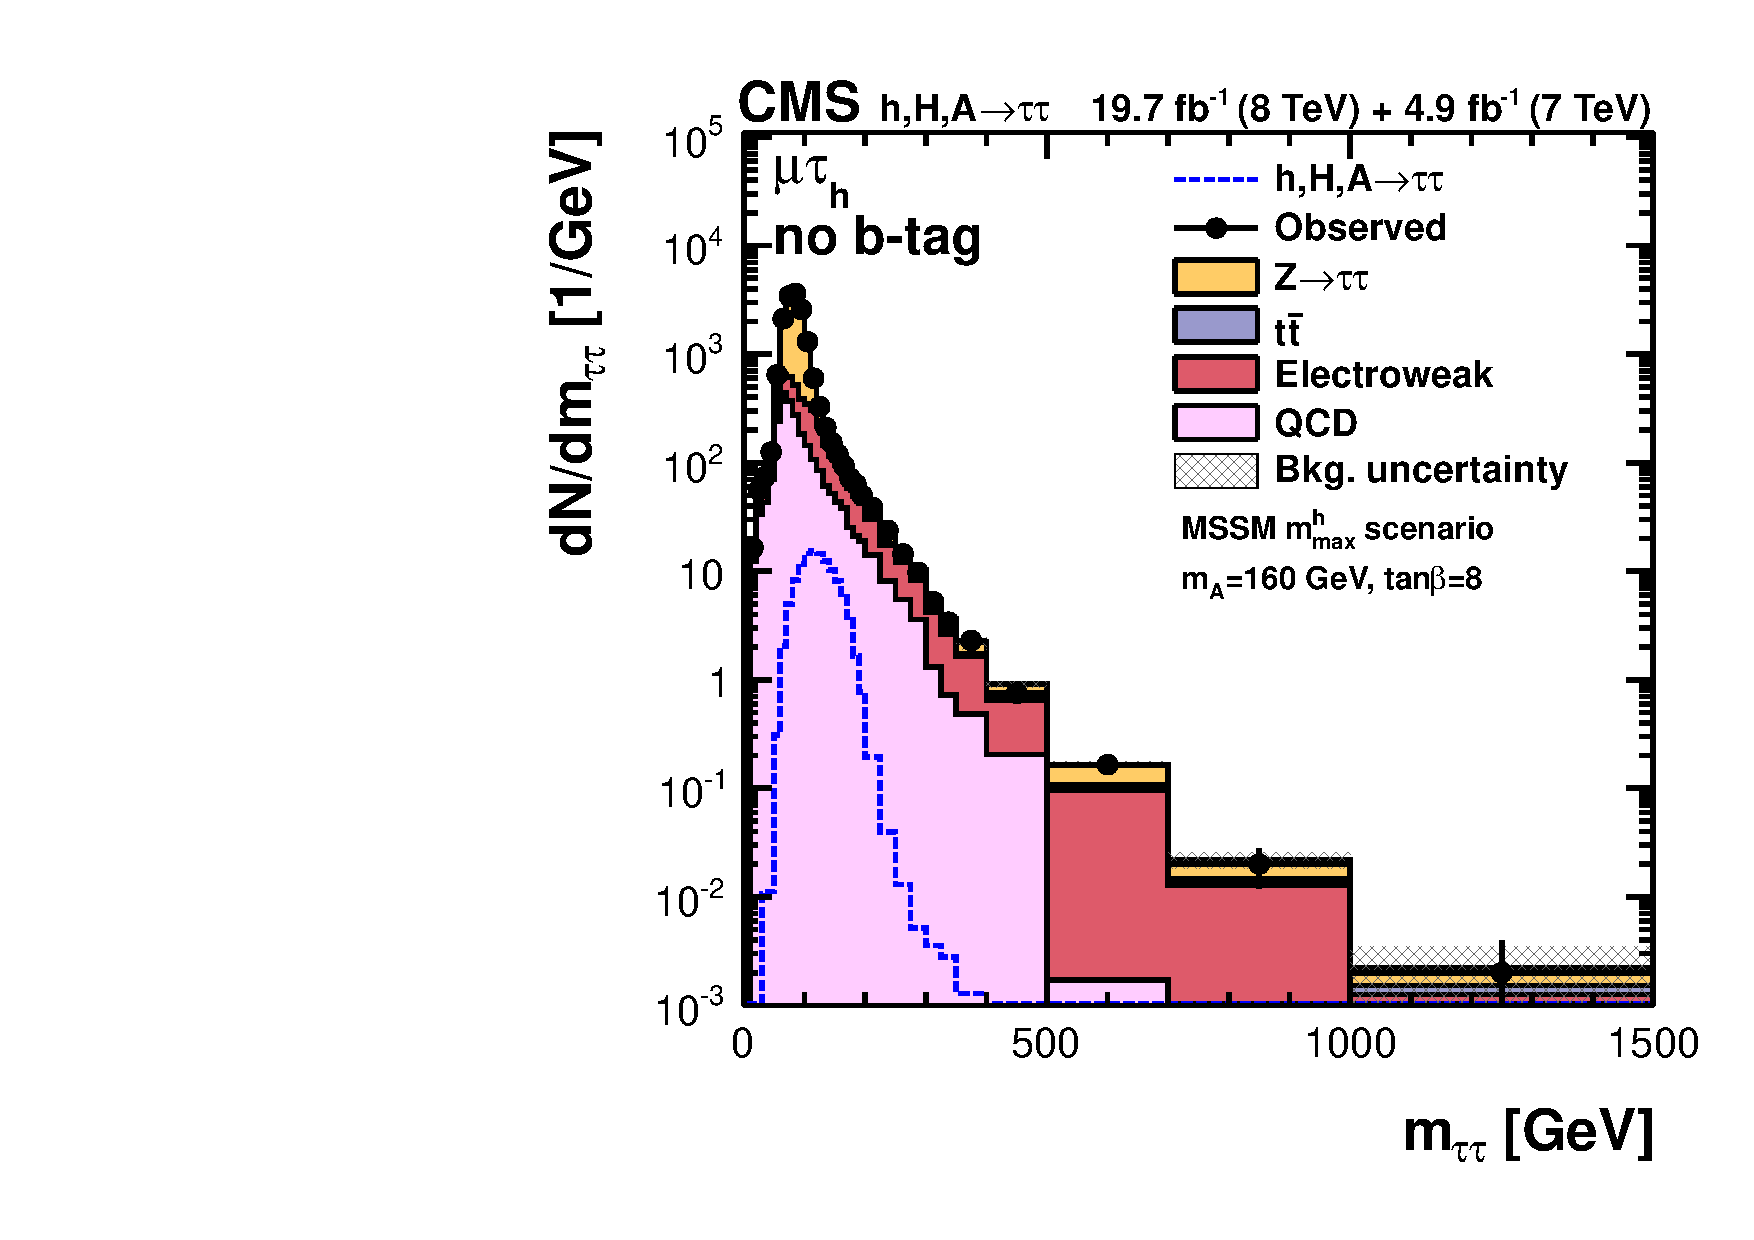
\includegraphics[width=0.5\textwidth]{plots/htt-mssm/muTau_nobtag_postfit_7TeV_8TeV_LOG.pdf}}
\subfloat[]{
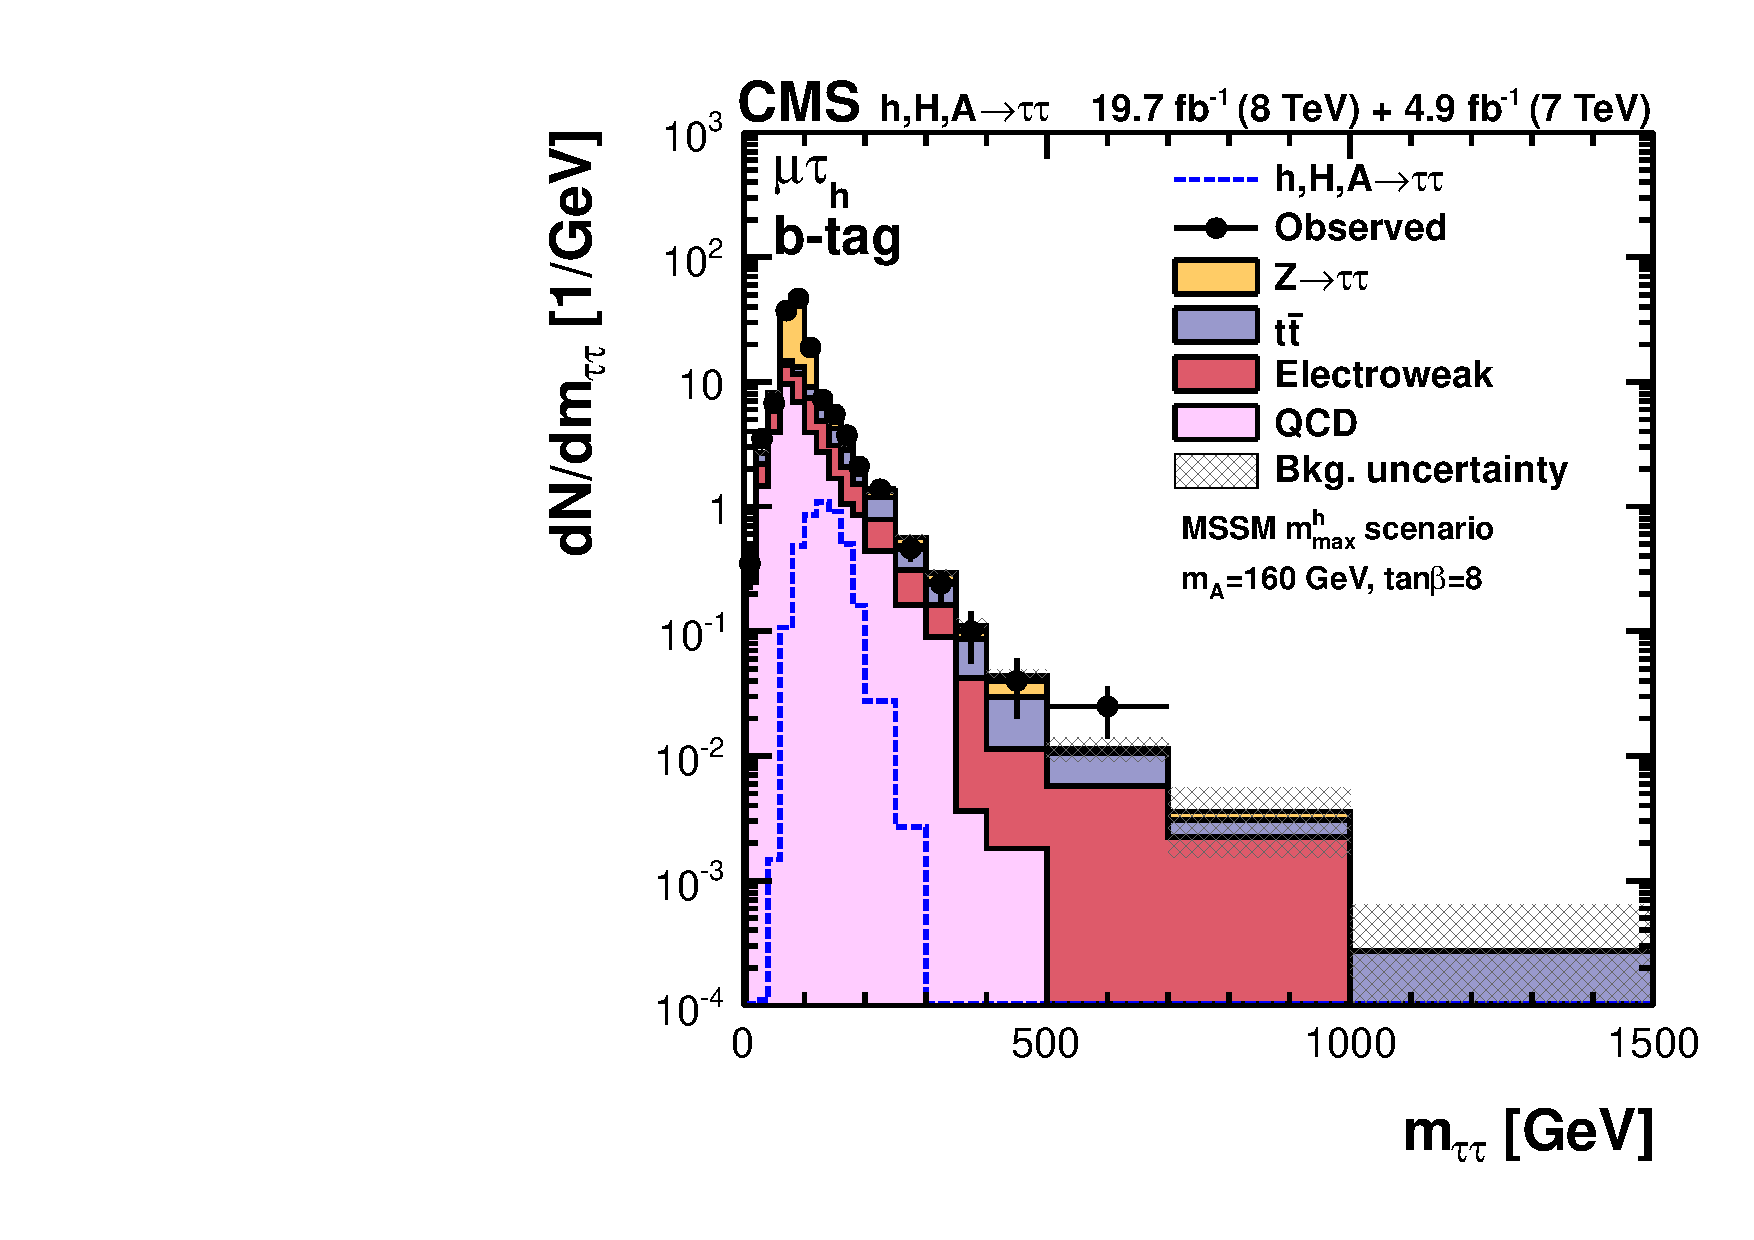
\includegraphics[width=0.5\textwidth]{plots/htt-mssm/muTau_btag_postfit_7TeV_8TeV_LOG.pdf}}

\subfloat[]{
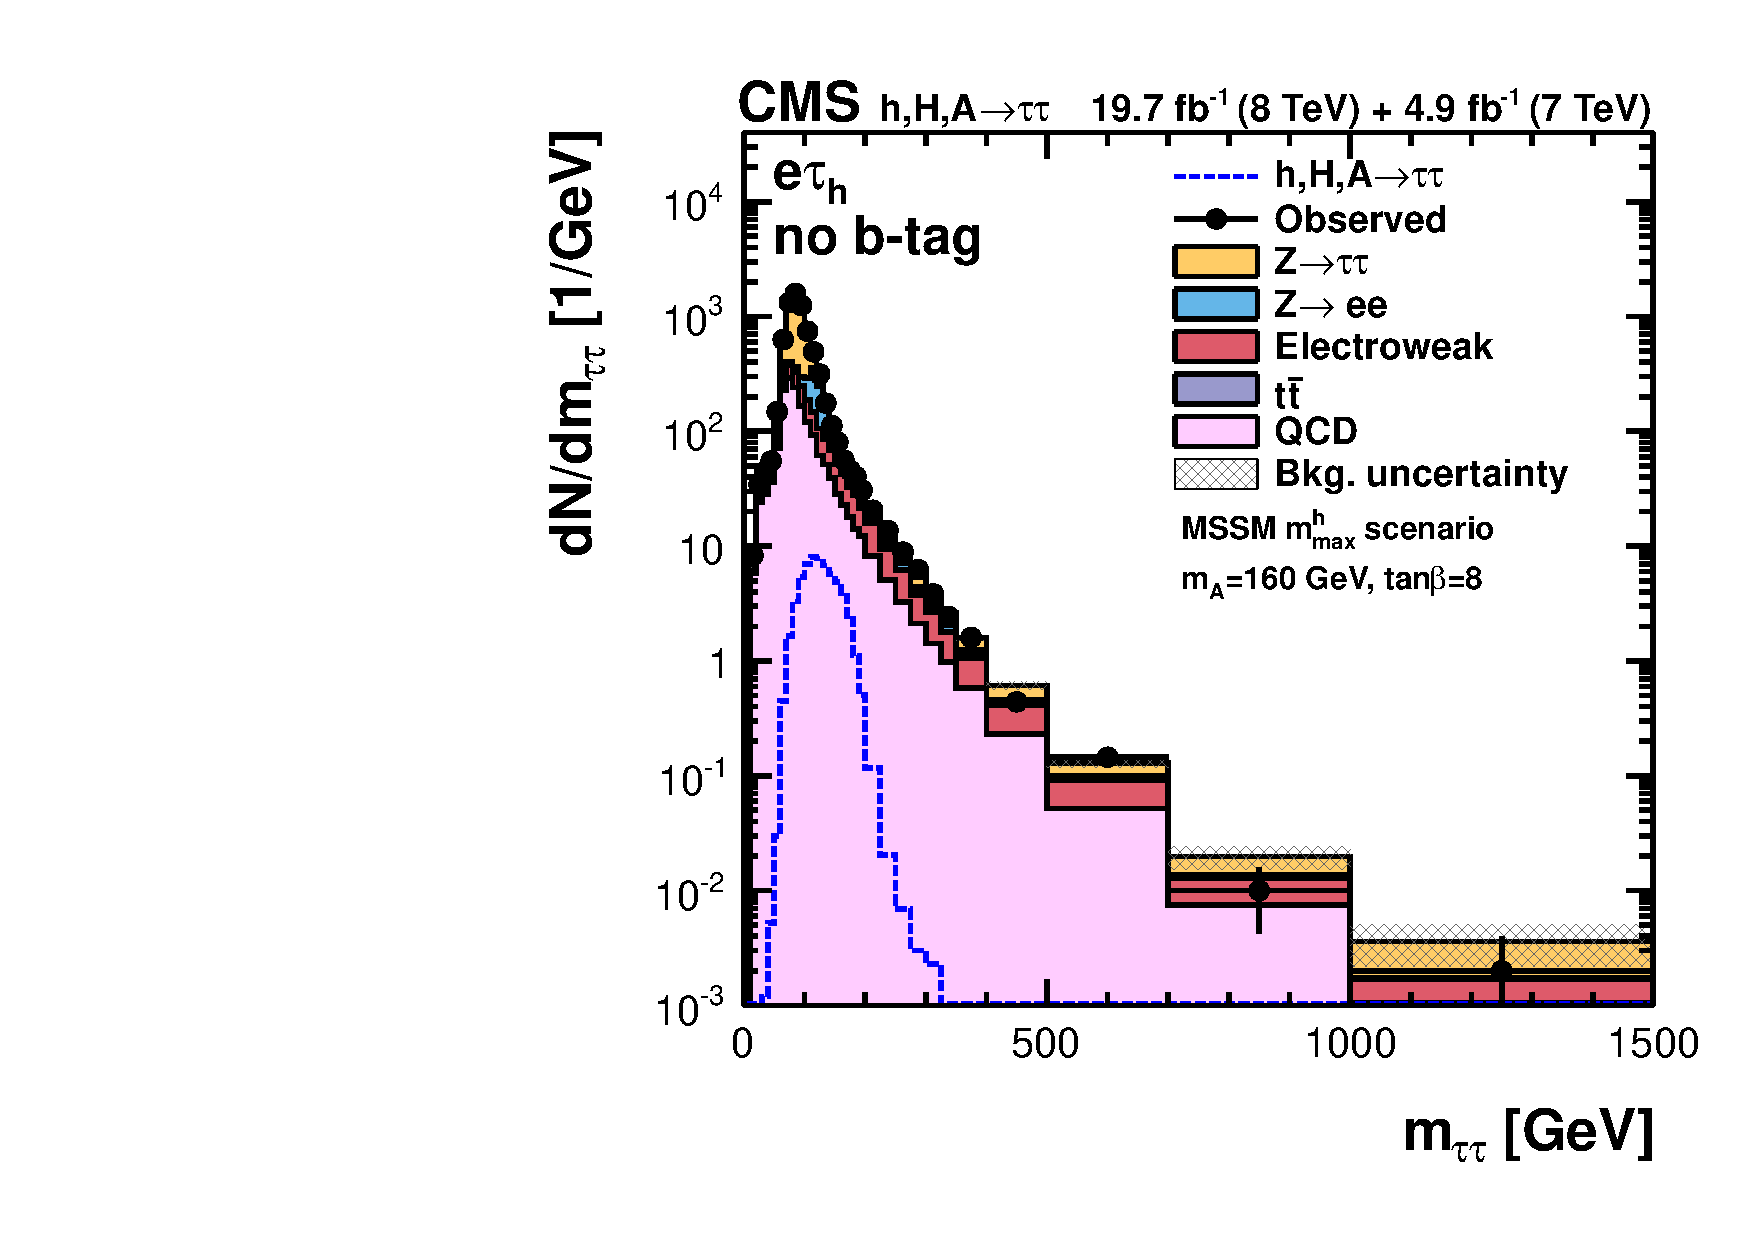
\includegraphics[width=0.5\textwidth]{plots/htt-mssm/eleTau_nobtag_postfit_7TeV_8TeV_LOG.pdf}}
\subfloat[]{
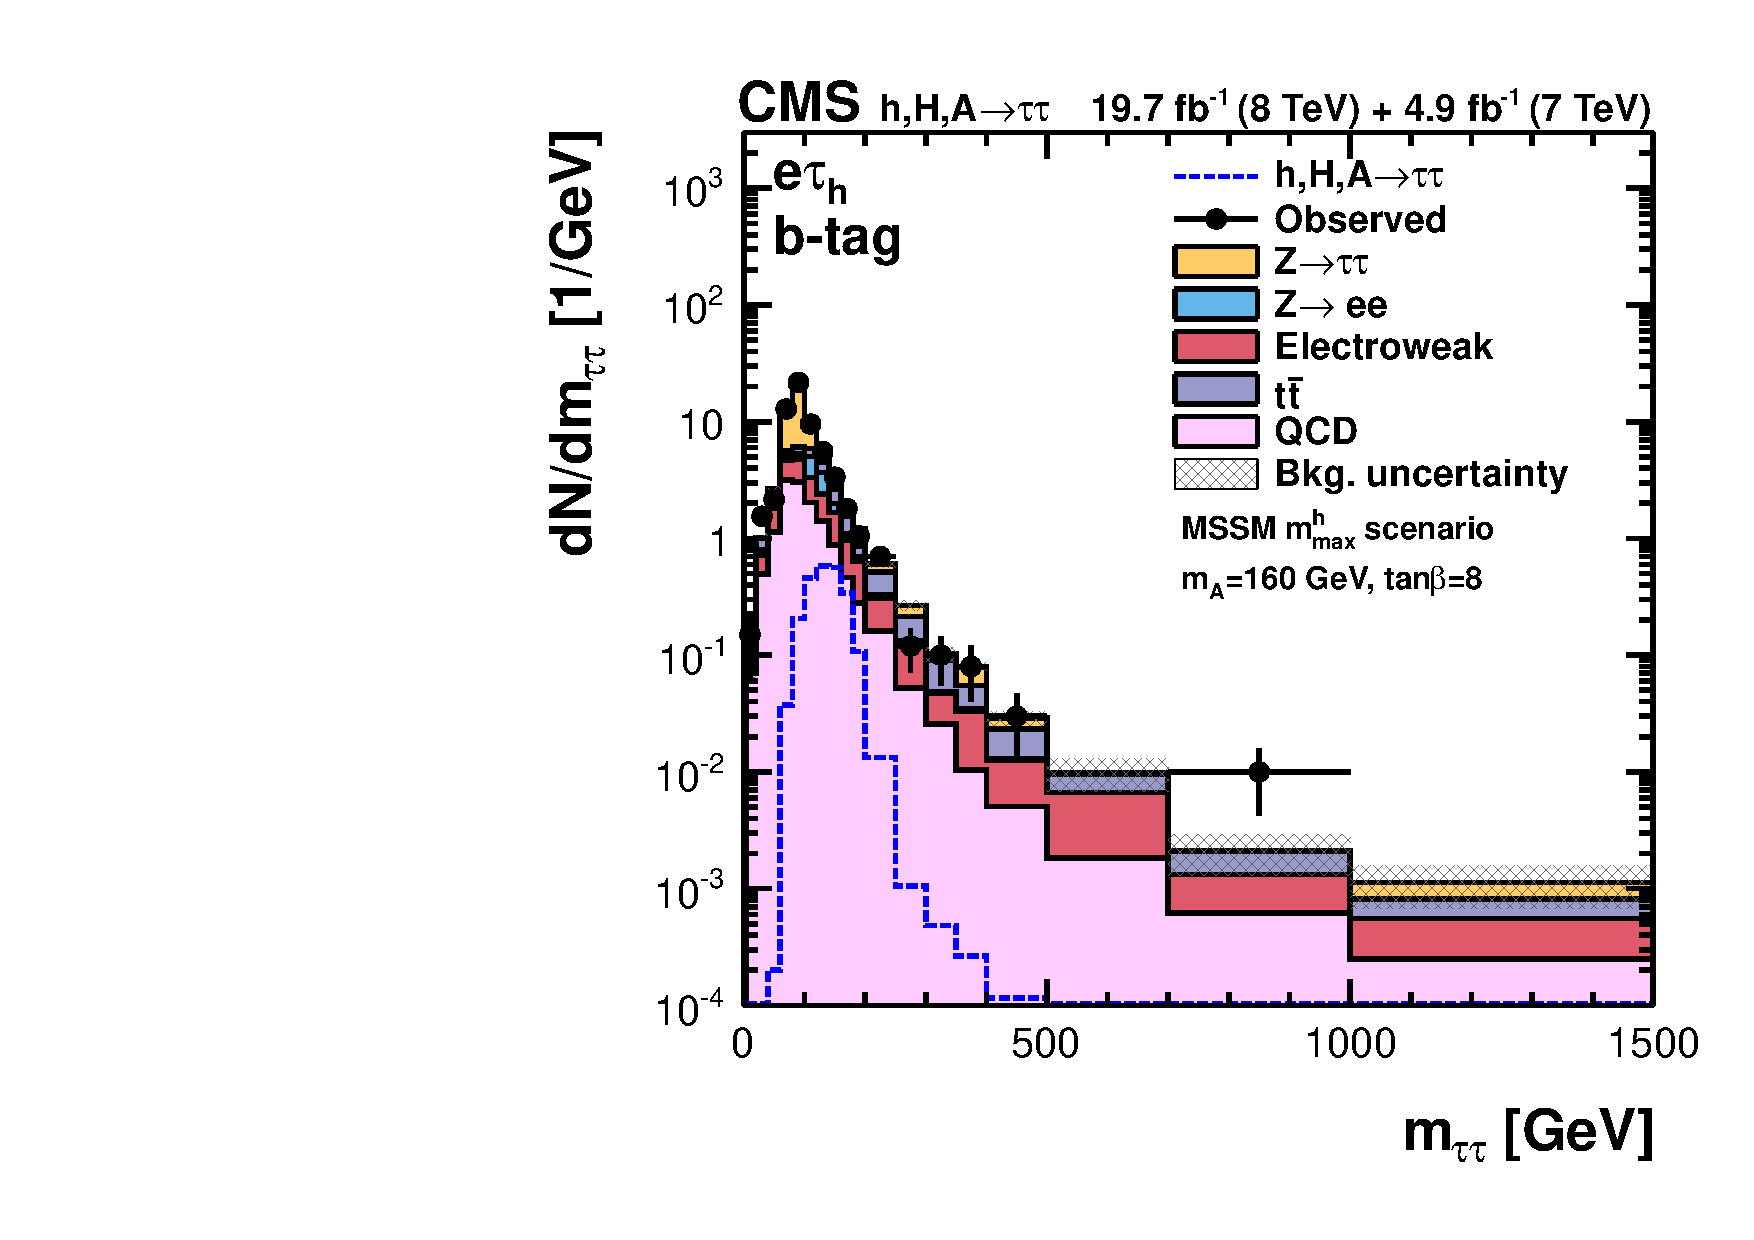
\includegraphics[width=0.5\textwidth]{plots/htt-mssm/eleTau_btag_postfit_7TeV_8TeV_LOG.pdf}}
\caption{Post-fit $m_{\Pgt\Pgt}$ distributions for the no-btag
(left) and b-tag categories. Plots are shown for
the $\mutau$ channel (top) and $\etau$ channel (bottom) \cite{}.}
\label{fig:mssmpostfitmass}
\end{figure}



\subsection{Signal Extraction}

\subsection{Model Independent limits}

\subsection{Model Dependent limits}

\subsubsection{Benchmark scenarios}




